\chapter{Thiết kế và triển khai hệ thống}
\section{Tách phát hiện khỏi theo dõi}
\begin{figure}[htbp]\centering
\fbox{\begin{minipage}{0.87\linewidth}\centering
Video và nhãn theo từng camera\\[3pt]
$\downarrow$\\
Bộ phát hiện YOLO $\longrightarrow$ bộ nhớ đệm theo video\\[3pt]
$\downarrow$\\
Lọc theo lớp và điểm $\longrightarrow$ ByteTrack + bộ lọc chuyển động\\[3pt]
$\downarrow$\\
Quỹ đạo có ID $\longrightarrow$ TrackEval $\longleftarrow$ nhãn chuẩn
\end{minipage}}
\caption{Đường đánh giá trên máy tính. Mỗi checkpoint có một bộ nhớ đệm dùng chung cho các bộ lọc trong phép so.}
\end{figure}
Mỗi video có ba loại dữ liệu với vai trò riêng. Ảnh là đầu vào của detector, phát hiện là đầu vào của tracker, còn nhãn chuẩn (GT) dành cho bộ chấm. Cách phân tách này cho phép quay lại một khung hình để hỏi detector có tìm thấy xe hay không trước khi quy lỗi cho bộ lọc. Trong benchmark dùng detector thật, tracker không đọc GT. Phép thử dùng hộp sinh từ GT được đánh dấu và phân tích riêng.

\section{Xây dựng dữ liệu huấn luyện}
Hai nguồn hình ảnh bổ sung cho nhau. BDD100K cung cấp cảnh từ phương tiện đang di chuyển, có năm lớp mục tiêu gồm ô tô, xe tải, xe buýt, xe máy và xe đạp. Phần UA-DETRAC bổ sung góc quan sát giao thông từ camera cố định. Việc chia theo video giữ các khung lân cận trong cùng một tập. Nếu hai khung gần như trùng ảnh xuất hiện ở hai phía của phép chia, điểm phát triển có thể phản ánh mức quen thuộc với một cảnh cụ thể.

\begin{table}[htbp]\centering
\caption{Thành phần tập mixed5 sau khi chọn khung hình. Số hộp là tổng nhãn dương của năm lớp.}\label{tab:train}
\begin{tabular}{llrrr}\hline
Nguồn & Phần & Video & Ảnh & Hộp\\\hline
BDD100K & Huấn luyện & 1.261 & 50.487 & 428.435\\
UA-DETRAC & Huấn luyện & 48 & 6.556 & 47.627\\
BDD100K & Phát triển & 139 & 5.559 & 46.799\\
UA-DETRAC & Phát triển & 12 & 1.631 & 11.561\\\hline
\end{tabular}
\end{table}
Tập huấn luyện gồm 57.043 ảnh trên 1.309 video. Phần UA-DETRAC lấy khung có nhãn theo bước mười. Các vùng bỏ qua được tô xám, còn phần hộp có nhãn được bảo toàn khi xuất dữ liệu. Trong huấn luyện, \emph{van} được gộp vào ô tô và \emph{others} vào xe tải. Ánh xạ thứ hai mang sai số ngữ nghĩa vì lớp gốc có thể gồm nhiều loại xe. Tập phát triển gồm 7.190 ảnh trên 151 video. Bốn mươi video kiểm tra UA-DETRAC nằm ngoài cả hai phần.

\begin{figure}[htbp]\centering
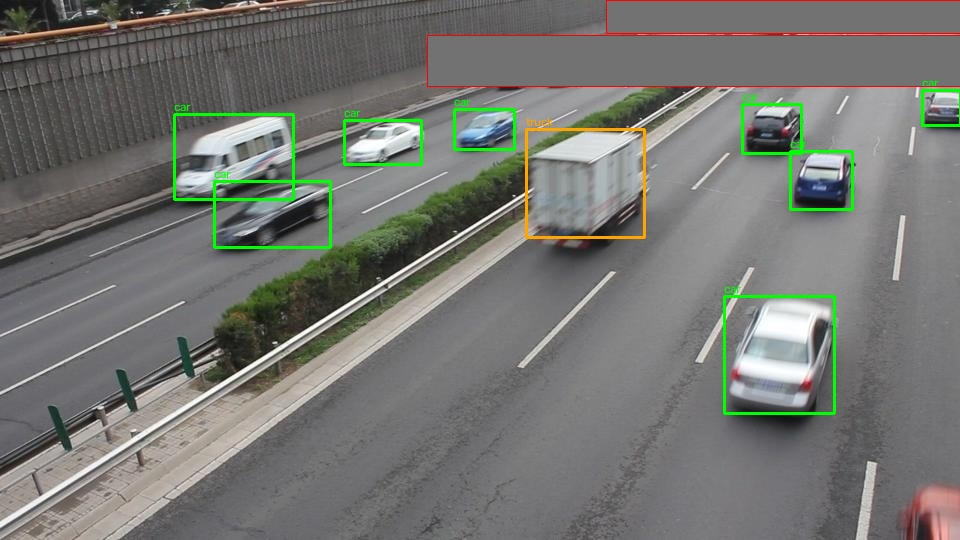
\includegraphics[width=0.8\linewidth]{hinh/detrac-train.jpg}
\caption{Ảnh huấn luyện UA-DETRAC, video MVI\_40241, khung 730, sau khi xuất nhãn mixed5. Hộp là nhãn dùng huấn luyện; các vùng xám đánh dấu phần bỏ qua. Nguồn ảnh và quy tắc chuyển đổi ở hồ sơ R52.}
\end{figure}
Phân bố lớp lệch mạnh về ô tô. Trong 476.062 hộp train, có 427.864 hộp ô tô nhưng chỉ có 2.235 hộp xe máy, đều thuộc BDD. UA-DETRAC không cung cấp nhãn riêng cho xe hai bánh. Một xe máy không có nhãn trong ảnh huấn luyện có thể trở thành ví dụ nền đối với detector. Vì thế, chất lượng ô tô không thể đại diện cho chất lượng xe máy. Nguồn nhãn train BDD là bản đóng gói lại đã ghim phiên bản và kiểm tra nội dung, chưa đối chiếu được với archive train gốc.

\section{Ba bộ phát hiện}
YOLOv8n COCO dùng trọng số gốc làm mốc. Hai detector còn lại, YOLOv8n mixed5 và YOLO11n mixed5, được khởi tạo từ trọng số COCO rồi huấn luyện 15 epoch trên tập trộn. Checkpoint dùng ở các vòng sau được chọn trên tập phát triển nội bộ, tương ứng epoch 15 và epoch 13. Đổi từ YOLOv8n COCO sang YOLOv8n mixed5 đồng thời đổi trọng số học được và không gian lớp. Điểm của cặp này đo kết quả của hai cấu hình hoàn chỉnh. Nó không cho biết mức cải thiện riêng do trộn thêm ảnh từ UA-DETRAC.

Đánh giá detector chạy FP32, kích thước danh nghĩa 640, ngưỡng thu nhận 0,001, NMS theo lớp ở IoU 0,7 và tối đa 300 hộp. Điểm precision và recall vận hành dùng ngưỡng 0,25. Đường tracking có cache riêng sinh ở ngưỡng 0,05. Với UA-DETRAC, đường sinh cache cho phép tới 3.000 hộp trước bước lọc lúc đọc để tránh cắt mất ứng viên sớm. Tên lớp của mô hình năm lớp được chuyển về ID COCO trước khi lọc. Hệ thống giữ thứ tự phát hiện sau NMS để các bộ lọc đối mặt với cùng bài toán gán.

\section{Cấu hình tracker và xử lý thời gian}
Hai điều kiện đầu vào được ký hiệu c25 và c10. Chúng giữ hộp có điểm lần lượt \emph{lớn hơn} 0,25 hoặc 0,10. ByteTrack giữ ngưỡng cao 0,25, ngưỡng thấp 0,10 và ngưỡng khởi tạo 0,25. Vòng ghép đầu dùng chi phí kết hợp IoU với điểm phát hiện, chấp nhận tới ngưỡng 0,8. Do đó ở c25, mọi hộp dưới ngưỡng cao đã bị loại từ đầu và vòng ghép điểm thấp rỗng. Ở c10, nhiều hộp có thể đi tiếp vào vòng này. Thêm ứng viên vừa có thể cứu một quỹ đạo vừa có thể tạo phép ghép sai, nên chênh lệch c10 và c25 cần đọc ở mức cấu hình.

Mỗi bộ lọc cung cấp cùng các thao tác khởi tạo, dự đoán và cập nhật. Cấu hình KF dùng trạng thái tám chiều. EKF và UKF dùng trạng thái chín chiều, cùng hàm chuyển CTRV và phép chiếu hộp. PF500 cơ sở dùng 500 hạt trên mỗi quỹ đạo, lấy mẫu lại theo ESS, tắt nhiễu bổ sung sau lấy mẫu lại và tắt đề xuất tối ưu. Hạt và bộ sinh ngẫu nhiên thuộc riêng từng quỹ đạo. Seed gốc cùng mã video và ID quyết định chuỗi số ngẫu nhiên. Ba seed 0, 1, 2 kiểm tra biến thiên khi chạy lại cùng cấu hình.

Biến thể PF500 K1/K2 dùng cho một số phép đối chiếu sau. K1 lấy mẫu lại các tọa độ quan sát từ phân bố Gauss điều kiện của từng hạt khi có phép đo. K2 thêm nhiễu sau lấy mẫu lại, với hệ số riêng cho phần hộp và phần chuyển động. Cấu hình motion2 nhân đôi hệ số nhiễu của nhóm biến chuyển động so với hệ số cơ sở của K2. Khi mất quan sát, bước dự đoán dựa vào trạng thái và nhiễu quá trình. Các bảng sau ghi rõ biến thể PF để tách các phép so với benchmark cơ sở.

Thời gian chờ khi mất dấu xấp xỉ 1,2 giây. Với UA-DETRAC ở 25 fps, giới hạn là 30 bước. Với BDD100K ở 5 fps, giới hạn chỉ còn 6 bước. Cùng hai bước liên tiếp ở hai tập tương ứng với hai khoảng thời gian vật lý khác nhau. Bộ lọc dự đoán theo bước ảnh và giữ đơn vị vận tốc theo bước. Khung hình không có phát hiện vẫn có vị trí trên trục thời gian theo giao thức của từng tập. Nếu loại các khung trống rồi đánh số liên tục lại, một khoảng mất quan sát sẽ bị rút ngắn giả tạo.

\subsection{Đề xuất có điều kiện đo trong PF}
Gọi $f_{ij}$ là tọa độ thứ $j$ sau mô hình chuyển của hạt $i$, $q_{ij}^2$ là phương sai quá trình theo tọa độ đó và $r_j^2$ là phương sai đo. Trong triển khai K1, bốn tọa độ $c_x,c_y,a,h$ có phép đo tuyến tính và nhiễu chéo. Phân bố dùng lấy mẫu tại những tọa độ này có phương sai và trung bình
\begin{align}
 s_{ij}^{2}&=\left(\frac{1}{q_{ij}^{2}}+\frac{1}{r_j^{2}}\right)^{-1},\\
 m_{ij}&=s_{ij}^{2}\left(\frac{f_{ij}}{q_{ij}^{2}}+\frac{z_j}{r_j^{2}}\right).
\end{align}
Sau đó $x_{ij}$ được lấy từ $\mathcal{N}(m_{ij},s_{ij}^2)$. Các tọa độ chuyển động tiếp tục dùng mẫu đã dự đoán. Hệ số cập nhật trọng số dựa vào mật độ dự đoán của phép đo, với log-mật độ bỏ hằng số chung
\[
 \ell_i=-\frac12\sum_{j\in\{c_x,c_y,a,h\}}
 \left[\frac{(z_j-f_{ij})^2}{q_{ij}^2+r_j^2}
       +\log(q_{ij}^2+r_j^2)\right].
\]
Phương sai quá trình phụ thuộc kích thước hộp từng hạt, nên số hạng log-phương sai được giữ. Thuật toán ép chiều cao dương sau lấy mẫu và chuẩn hóa trọng số trong miền log. Mục đích của K1 là sử dụng quan sát hiện tại khi đặt các mẫu ở phần trạng thái quan sát được, qua đó hạn chế tình trạng nhiều hạt được dự đoán ra xa phép đo. Hiệu quả giữ ID còn phụ thuộc việc tracker có ghép được phép đo cho quỹ đạo trước khi cập nhật.

\subsection{Theo dõi vòng đời và xử lý mất quan sát}
Mỗi quỹ đạo có thể đang hoạt động, đang mất dấu hoặc đã bị loại. Trong một khung, hệ thống thực hiện lần lượt các bước sau.
\begin{enumerate}
\item Giữ vị trí của khung trong dòng thời gian, đọc các phát hiện và lọc lớp, điểm theo giao thức.
\item Dự đoán trạng thái của các quỹ đạo thuộc nhóm được xét ghép.
\item Tính chi phí giữa hộp dự đoán và hộp quan sát, giải bài toán gán với ngưỡng của vòng đầu.
\item Thử ghép các quỹ đạo đang hoạt động còn đủ điều kiện với phát hiện điểm thấp, rồi xử lý quỹ đạo chưa được xác nhận.
\item Cập nhật bộ lọc ở các cặp ghép thành công, khởi tạo từ phát hiện còn lại đủ điểm, đánh dấu mất và loại những quỹ đạo hết thời gian chờ.
\item Ghi kết quả theo frame, ID và hộp trong hệ tọa độ ảnh gốc.
\end{enumerate}
Đối với khung thiếu phát hiện, dự đoán vẫn làm tăng tuổi mất dấu. Bộ lọc có thể đưa ra hộp dự báo trong khoảng này, còn quyết định ghi một quỹ đạo vào đầu ra do quy tắc vòng đời chi phối. Vì thế, cần kiểm cả bước bộ lọc lẫn việc quỹ đạo còn được xét ghép ở khung tái xuất hiện.

\section{Thiết kế phép so và kiểm tra tái lập}
Trong mỗi tập đánh giá chính, ba detector nhân hai ngưỡng nhân sáu lượt bộ lọc tạo thành 36 lượt. Sáu lượt gồm ba cấu hình xác định và ba seed PF500. Mỗi lượt đọc tất cả video của tập. Sau khi chấm COMBINED riêng cho từng seed, nghiên cứu lấy trung bình ba điểm PF. Việc này khác với trộn quỹ đạo của ba seed rồi chấm một lần. Một seed cho kết quả cao cũng không thay thế được kết quả trung bình.

Trên UA-DETRAC test40, mỗi checkpoint có 40 đơn vị cache. Hệ thống chấm đủ 1.440 đơn vị lượt--video. Trên BDD val, 600 đơn vị cache cung cấp đầu vào cho 7.200 đơn vị lượt--video. Phép kiểm tính lặp lại trên BDD gồm lặp tracker cho 36 lượt trên video định trước và chấm lại sáu lượt, đều trùng byte với đầu ra được đối chiếu. Các kiểm tra này xác nhận đường xử lý lặp lại được trong môi trường đã ghi nhận. Chúng không thay thế khoảng tin cậy cho biến thiên giữa video.

Đối với hiệu số trong một nhóm detector và ngưỡng, bootstrap lấy lại video theo cặp. Ở mỗi lần lấy mẫu, cùng danh sách chỉ số video được dùng cho hai bộ lọc, rồi tổ hợp lại các thành phần điểm. Cách làm này giữ quan hệ giữa các bộ lọc cùng gặp một video khó. Trên BDD, ma trận lấy mẫu gồm 5.000 lần, mỗi lần có 200 vị trí video. Trên UA-DETRAC, phân tích còn xét 39 nhóm để thử độ nhạy với một cặp video có liên hệ trong thiết kế phân nhóm. Các khoảng riêng lẻ không có hiệu chỉnh đa so sánh.

\section{Đường triển khai Jetson Nano}
Trên Nano, detector TensorRT nhận ảnh đã đổi kích thước và thêm đệm. Kết quả sau suy luận được lọc và đưa vào phiên bản tracker NumPy. Đường chạy trực tiếp vừa phát hiện vừa theo dõi. Đường phát lại dùng phát hiện đã lưu rồi chạy cùng tracker. So sánh tệp quỹ đạo giữa hai đường giúp phát hiện lỗi chuyển tọa độ, thứ tự hộp hoặc bước cập nhật ngay cả khi video hiển thị trông hợp lý.

Các phiên bản KF và EKF dùng backend NumPy trong phép đo đầu vào engine. Phép đo 80 video của cấu hình mới sử dụng KF trực tiếp trên Nano. Sau đó cache phát hiện từ cùng engine được chấm với cả bốn bộ lọc trên PC. Chương~\ref{chap:nano} trình bày các phép đo theo giai đoạn và điều kiện chạy của từng phép so.
